\chapter{Introduction}
\label{sec:introduction}

The work in this thesis is concerned with the analysis of the rhythmic structure in performances of music. We will study rhythmic structure in isolation of other structures that may be present in the music like melody or harmony.

This chapter will introduce concepts used throughout this thesis and discuss related studies. First, rhythmic structure is introduced. Then in section \ref{sec:performances}, structure will be related to performance and finally in section \ref{sec:introducing} the approach presented in this thesis will be introduced.

The rest of this thesis is structured as follows: In chapter \ref{sec:method}, our approach will be described in detail. Chapter \ref{sec:method} will also introduce the annotated jazz corpus that was produced for this thesis. In chapter \ref{sec:evaluation}, we will describe how we intent to evaluate our system. Then in chapter \ref{sec:results} the system will be evaluated on the jazz corpus. Chapter \ref{sec:discussion} will discuss to what extent the system was successful based on the results and improvements will be suggested. Finally, chapter \ref{sec:conclusion} will present the conclusions of this thesis.

\section{Rhythmic Structure}
\label{sec:structure}

A rhythm, in most Western music traditions, is composed of metrical units, rests or notes, whose duration is specified relative to each other. A note tells the performer to play some pitch for the duration of the note, a rest indicates a silence for the duration of the rest. Durations are specified as subdivisions of the duration of a whole note: some common subdivisions are: half notes or rests, quarter notes or rests, eighth notes or rests, etcetera. Their notation in the so-called staff music notation is illustrated in table \ref{tab:notation}. Apart from the duple divisions mentioned above, triple divisions, quintuple and any other prime number divisions are allowed as well although divisions higher than triple are rare. 

\begin{table}
\caption{Some music notation conventions.}
\label{tab:notation}
\centering
\begin{tabular}{lllll}
\parbox{0.15\linewidth}{
\centering
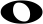
\includegraphics[scale=0.5]{img/whole_note}
}
&
\parbox{0.15\linewidth}{
\centering
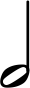
\includegraphics[scale=0.5]{img/half_note}
}
&
\parbox{0.15\linewidth}{
\centering
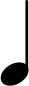
\includegraphics[scale=0.5]{img/quarter_note}
}
&
\parbox{0.15\linewidth}{
\centering
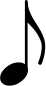
\includegraphics[scale=0.5]{img/eighth_note}
}
&
\parbox{0.15\linewidth}{
\centering
\includegraphics[scale=0.5]{img/meter}
}
\\
A whole note. & A half note. & A quarter note. & An eighth note & A 4/4 time signature\\

\end{tabular}
\end{table}

These durations are grouped together units called bars or measures. The time signature specifies how a bar is subdivided into metrical units. The time signature consists of two numbers written above each other as in table \ref{tab:notation}, when written in text we refer to this as a 4/4 time signature where the first number is the top number and the second number is the bottom number. The top number specifies the number of notes per measure, the bottom number specifies the units of those notes. The time signature is sometimes called meter.

Staff music notation is one of the most widespread representation of rhythmic structure. In the field of rhythm analysis, another structure is popular, called a \textit{metrical grid}, which originally introduced by \citet{lerdahl1983generative} in their Generative Theory of Tonal Music. A metrical grid is a representation that contains several levels, where the lowest level corresponds to the smallest subdivided unit and the highest level corresponds to a bar. A metrical grid representing a 3/4 time signature is shown in figure \ref{fig:grid}. Bars are separated using a horizontal line, $\bullet$ symbols indicate the \textit{downbeats} of each level. The downbeats are the leftmost units metrical unit of a subdivided unit. Level three for example contains one downbeat per bar. Level three is subdivided into three level-two downbeats, the second and third of which is a level-three \textit{upbeat}. Every level-two unit is subdivided into two level-one downbeats, the second of which is a level-two upbeat. 

\begin{figure}[b]
\centering
\hspace{2in}
\begin{tabular}{llllll|llllll|ll}
$\bullet$ &  &  &  &  &  & 		$\bullet$ &  &  &  &  &  & $\bullet$ & Level 3\\ 
$\bullet$ &  & 	$\bullet$ &  & 	$\bullet$ & & 	$\bullet$ & & $\bullet$ &  & $\bullet$ &  & $\bullet$ & Level 2\\
$\bullet$ & 		$\bullet$ & 		$\bullet$ & 		$\bullet$ & $\bullet$ & $\bullet$ & $\bullet$ & $\bullet$ & $\bullet$ & $\bullet$ & $\bullet$ & $\bullet$ & $\bullet$ & Level 1\\
\end{tabular}
\caption{Metrical grid of a 3/4 time signature.}
\label{fig:grid}
\end{figure}

Having now introduced two representations of rhythmic structure, we can turn to some the work done in this field. The most extensive recent study was conducted by \cite{temperley2010modeling}, where he studies the probabilistic properties of rhythmic structures in isolation. It is suggested that rhythm has some probabilistic characteristics that are shared to some extend by a wide range of musical styles. Temperley identifies a number of intuitions about rhythm that seem to be common-practice. These intuitions include the general tendency of onsets to fall on downbeats, the preference for onsets on upbeats to be preceded or followed by a note on the previous or next downbeat and the tendency of long notes to fall on downbeats. 

Temperley proposes six different models intended to be sensitive to these regularities. The adequacy of these models is evaluated by measuring their cross-entropy, using cross-validation on a corpus of European folk songs. Temperley's work shows that it is fairly easy to devise probabilistic models that differentiate common rhythms from less common rhythms. Intuitively, these models explain that not every pattern of onsets that can by described as a valid rhythmic structure will be perceived as a rhythm by humans. 

% Metrical grids?

\section{Performances}
\label{sec:performances}

Rhythmic structure in itself does not imply onsets in absolute time. The common way to relate a rhythmic structure to a performance is by assigning some real duration to a metrical unit. The amount of real time we assign to a metrical duration is usually called the \textit{tempo}. Given a tempo, a rhythmic structure can be converted to a set of \textit{idealised} onset times, also called metronomic onset times. 

When humans perform a rhythm, they deviate from the idealised onset times in several ways. Unless a metronome is used, the tempo will usually fluctuate as the performance progresses. Much of this fluctuation is intentional and is referred to as \textit{musical expression}. Apart from global tempo changes humans deviate from idealised onsets locally as well, even when a metronome is used. 

In general, it is thought that, depending on the competence of the performer, some proportion of this local deviation, is noise but a large proportion of it seems to be systematic. A study by \citet{palmer1989mapping} suggested that global tempo changes are mostly guided by conscious intention. Local deviations in timing and loudness seemed to be partly unconscious. Pianists were for example aware that they articulated certain beats but could not reliably tell whether they did so by playing them louder or by altering their timing. These findings suggest that it is to some extent not even possible to perform rhythm without expression.

It seems thus that whereas global tempo changes may be guided by conscious intentions of phrasing, local expression may be partially unconscious. Another study has shown that there is some regularity in local expression that is linked to rhythmic structure \citep{bengtsson1983analysis}. In Vietnamese waltzes for example, which have almost exclusively a 3/4 or 6/8 meter, it is observed that there is a consistent lengthening of the first upbeat at quarter note level.

Although a performance deviates from the idealised onsets given by the structure and tempo, human listeners are often able to derive the rhythmic structure from a performance and multiple listeners tend to be quite consistent in their interpretations of a performance. In fact, the studies above suggest that deviations from idealised onsets are crucial to perception of structure in rhythm.

%Much of this expression appears to be a highly complicated and irregular process that is influenced by factors as musical style and the `mood' of the music, the audience and the performer. There is a field of research concerned with finding models for musical expression, see for example \citet{widmer2004computational}. Here, we will not concern ourselves with extensive models of expression. Instead, we will suggest that there may be more regular forms of local expression that are the result of a tendency of humans to emphasize downbeats.

Several authors have suggested models that try to mimic this human capacity. \citet{cemgil2000rhythm} propose a system for rhythm quantisation that uses Bayesian modelling to derive the rhythmic structure. Their model tries to optimise the probability of a score given a performance, which can be expressed as the probability of the score (the score model) times the probability of the score given the performance (the rhythm model). The performance model simply penalises performances to the extent that they deviate from metronomic onset times. The model assumes tempo can change and uses a tempo-track (often called tempo-curve) to derive metronomic onset times given local tempo. 

\citet{raphael2002hybrid} proposes another model that is similar to the model in \citet{cemgil2000rhythm}. However, here a graphical probabilistic model is proposed where `score-positions' (relative positions of notes within a measure) are seen as a Markov chain of events where the probability of a score position depends on the probability of a note on that position and the probability of a note on that position preceded by the score-position of the previous note. Another Markov chain of tempo values is generated from the the score positions and finally the exact onset time of each note is dependent on the tempo value, score position of the previous note and score position of the current note.

These models are discussed in \citet{temperley2007music} and it is observed that the actual metrical structure still remains ambiguous in the analyses of these models. Temperley proposes a model of rhythm here that is based on a metrical grid, an unambiguous representation of meter and also contains less parameters than the rather complicated models of \citet{raphael2002hybrid} and \citet{cemgil2000rhythm}. This model is elaborated in \citet{temperley2009unified} where it is integrated into a unified probabilistic model of rhythm, harmony and polyphonic structure.

In this study, a rhythm model is proposed implemented based on what Temperley calls metrical anchoring: the probability of a beat on an upbeat depends on whether a note was played on the preceding or following downbeat, this model is called the hierarchical model by Temperley. Later, in \citet{temperley2010modeling}, this model is compared to other rhythm models and it is shown that it performs adequately. This rhythm model is also based on the notion of a metrical grid and is limited to metrical grids containing four levels and only duple divisions. To deal with the problem of tempo, the model has a parameter that specifies the preferred \textit{tactus level} interval. The tactus level is the level in the metrical grid that corresponds to the beats in a measure (see our discussion of time signatures in section \ref{sec:structure}). The tactus interval is allowed to fluctuate: the probability of a next tactus interval is a normal distribution over the previous one, preferring tactus intervals of the same length.

The notion that rhythmic structure is, as it was suggested before, always performed expressively has been largely ignored by the models described above. In all models, expression was considered additive noise with respect to the idealised onsets given some rhythmic structure and tempo representation. Another criticism of the models above is that they all include one or more parameters that are related to tempo. Estimating local tempo is not trivial: in the case of slightly stretched beats as the result of local expression, the beats following that beat will be considered to deviate from the average tempo of that measure. Defining tempo per beat, seems tedious and hard to do accurately. This may lead us to believe that the concept of tempo in relation to expressively performed rhythms may be misleading. A related view is put forward by \citet{desain1993tempo}, who argue that tempo curves can be misleading concept.

In the next section, we will introduce a model that is completely tempo independent and has the potential to become sensitive to rhythmic structure-dependent local expression.

\section{An Expression-Aware Subdivision-Based Rhythmic Parser}
\label{sec:introducing}

% Therefore we present our expression model the way it is presented

% This approach is based on early work by longuet-higgins.
% We try to use regular expression to our advantage
% Also tempo tracks are weird, given that rhythms are always performed expressively and introduce lots of parameters
% Temperleys unified analysis is cool but also estimates a tactus level that is based on real times and it needs 'pips'
% A performance of Chopin includes huge tempo changes that can be instantaneous. A model needs to be free of any assumptions about tempo.

The approach introduced here is inspired by \citet{longuet1976perception}. In this work, rhythmic structure is represented as subdivision trees rather than staff notation or metrical grids. A subdivision tree represents rhythms as a hierarchical structure where some metrical duration corresponding to the root node is subdivided into child nodes. An example of such a structure is shown in figure \ref{fig:subdivision:a} and three possible staff notation interpretations of the structure in figure \ref{fig:subdivision:b}. Although musicians might play score C slower than score B and score B slower than score A, they are structurally identical and as we have said earlier, our model will be tempo-independent. The different scores are inferred from the tree by defining some level in the tree to be the bar duration.

\begin{figure}[t]
\centering
\subfloat[]{
\label{fig:subdivision:a}
\centering
\Tree
[ .{$\frac{1}{1}$} [ .{$\frac{1}{2}$} [ .{$\frac{1}{4}$} [ .$\bullet$ ] [ .{$\frac{1}{8}$} [ .$\bullet$ ] [ .$\bullet$ ] [ .$\bullet$ ] ] ] [ .{$\frac{1}{4}$} [ .$\bullet$ ] [ .$\bullet$ ] ] ] [ .{$\frac{1}{2}$} [ .{$\frac{1}{4}$} [ .$*$ ] [ .$\bullet$ ] ] [ .$\bullet$ ] ] ] 
}

\subfloat[]{
\label{fig:subdivision:b}
\centering
\begin{tabular}{| l  >{\arraybackslash}m{2.3in} |}
\hline 
A & 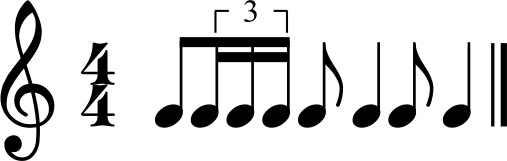
\includegraphics[scale=0.3]{img/subdivision_score1}\\
B & 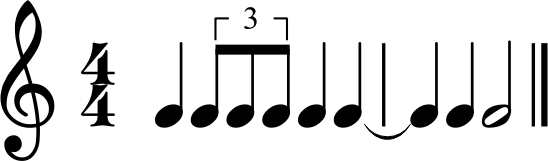
\includegraphics[scale=0.3]{img/subdivision_score2}\\
C & 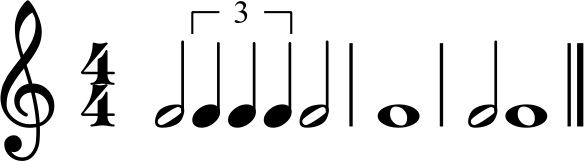
\includegraphics[scale=0.3]{img/subdivision_score3}\\
\hline
\end{tabular}
}
\caption{An analysis and three different score notations of the same musical clich\'e. }
\label{fig:subdivision}
\end{figure}

In staff notation the longest metrical unit is a whole note, which can be lengthened using dotted notation or ties. In the subdivision tree in figure \ref{fig:subdivision}, every node represents some metrical duration which may correspond to notes, bars or multiple bars. Although figure \ref{fig:subdivision} only shows duple and triple subdivisions a metrical unit in the tree can be subdivided into any prime number child-units. We specify two types of leaf-nodes: an onset, which we show as a $\bullet$ symbol in subdivision trees and a tied note, which we show as a $*$ symbol in subdivision trees. Figure \ref{fig:ties} shows how these symbols are interpreted. The $\propto$ symbol means that the expression on the left is proportional to the expression on the right.

\begin{figure}
\centering
\subfloat[A subdivision of a three note rhythm.]{
\parbox{0.25\linewidth}{
\centering
\Tree
[ .{$\frac{1}{1}$} [ .$\bullet$ ] [ .{$\frac{1}{2}$} [ .$\bullet$ ] [ .$\bullet$ ] ] ]
}
$\mathlarger{\mathlarger{\mathlarger{\propto}}}$
\parbox{0.25\linewidth}{
\centering
\includegraphics[scale=0.3]{img/intro1}
}
}

\subfloat[A subdivision tree of a two note rhythm containing a tied note.]{
\parbox{0.25\linewidth}{
\centering
\Tree
[ .{$\frac{1}{1}$} [ .$\bullet$ ] [ .{$\frac{1}{2}$} [ .$*$ ] [ .$\bullet$ ] ] ]
}
$\mathlarger{\mathlarger{\mathlarger{\propto}}}$
\parbox{0.25\linewidth}{
\centering
\includegraphics[scale=0.3]{img/intro2}
}
}
\caption{The interpretation of onsets and ties in subdivision trees.}
\label{fig:ties}
\end{figure}

The approach presented in \citet{longuet1976perception} is a rule-based system that needs to be initialised with a tactus length and some tolerance parameter that specified how much performances where allowed to deviate from metronomic timing. Nowadays, computers are powerful enough to construct probabilistic models based on corpora and to consider a great number of possible structural interpretations of a performance at once. With this in mind, we will briefly introduce our system below before discussing it in detail in the next chapter.

We will boil down a performance to a list of onsets. We think onsets provide enough information to correctly identify rhythmic structure. Therefore, we will from now on talk about onsets rather than notes.

Subdivision trees that describe valid rhythmic structures can be described in a context-free grammar (CFG). An algorithm that determines the hierarchical structure of an input given some CFG is called a parser. We will present a CFG and a parser that constructs hierarchical structures like in figure \ref{fig:subdivision:a} from performances. Our parser will be some variant of a class of efficient parsers called chart-parsers.

Our parser will be guided by a Bayesian model which allows us to describe a probable structure given a performance as the probability of the structure itself, described by a \textit{rhythm model} times the probability that this structure generated the observed performance, described by an \textit{expression model}.

Similar to \cite{temperley2009unified}, we will use a rhythm model that is sensitive to common-practice notions about rhythm. However, instead of his hierarchical model, which is based on metrical grids, we will use a probabilistic context-free grammar (see section \ref{sec:prior}). This model follows naturally from our representation of rhythmic structure.

We have claimed that some structure-related expressive deviations may be regular. Emphasising beats can result in a slight stretching of the duration of the beat. Depending on the style of the music, some beats may be emphasised regularly. In general it seems downbeats are often emphasised. If such stretching does indeed happen regularly, it will result in downbeats at levels near the leaf nodes of the tree to be slightly longer than upbeats. A tempo independent way to look at this is as the ratio of downbeat length and upbeat length. The expression model will assume that the down-/upbeat length ratio can be estimated from a number of features.

To train our rhythm and expression model, we need a corpus of monophonic performances of rhythms annotated with subdivision trees. For this purpose we have constructed a corpus of monophonic jazz melodies, performed by amateur musicians. The corpus was annotated with metrical onset times and subdivision trees were generated using a non-probabilistic version of our parser. This was possible because we could assume the onset times were metronomic.\footnote{Technically, the onsets are specified in metrical units and not metronomic units. However, since our parser is tempo-independent this does not matter.}

Finally, the parser is evaluated on the same corpus. We will use cross-validation to avoid testing on the same data we trained on.
%Representation: subdivision trees
%Context free grammar, parser
%Bayesian model: rhythm model, expression model
%Parameters learned from annotated corpus.
%Expression model: expression ratio
%Advantage of subdivision trees with respect to expression: we always know what the down- and upbeats are.